%%%%%%%%%%%%%%%%%%%%%%%%%%%%%%%%%%%%%%%%%
% v1.0.0
% lab-report-template
%%%%%%%%%%%%%%%%%%%%%%%%%%%%%%%%%%%%%%%%%

\documentclass[twocolumn]{article}

% Include packages and document structure

\usepackage[utf8]{inputenc}
\usepackage[a4paper,
            bindingoffset=0.2cm,
            left=1cm,
            right=1cm,
            top=1cm,
            bottom=2cm,
            footskip=1cm]{geometry}

\usepackage{lipsum}
\usepackage[italian,english]{babel}

\usepackage{graphicx} % Required to include images
\usepackage[labelfont=sc]{caption} %DT$18/02/2021 caption style
\usepackage{float} %DT$03/01/2020 better image positioning
\usepackage{cuted} %DT$29/07/2022 allows writing over the whole page

\usepackage{braket} % DT$13/11/2021 qm symbols
\usepackage{enumerate} % Custom item numbers for enumerations
\usepackage{placeins} %DT$04/01/2020 \FloatBarrier 
\usepackage{color} % Required for custom colors
\usepackage{amsmath,amsfonts,stmaryrd,amssymb,theorem} % Math packages
\usepackage{siunitx} %DT$03/01/2021 symbols ex:\SI{50}{\micro\second}
\sisetup{range-phrase={\text{\ -\ }},
     input-decimal-markers={.}, 
     range-units = single,
     output-decimal-marker = {.},
     group-digits=false}

\usepackage{booktabs}

\newcommand{\reffig}[1]{Figure~\ref{#1}}
\newcommand{\reftab}[1]{Table~\ref{#1}}
\newcommand{\refeqn}[1]{Equation~\ref{#1}}
\NewDocumentCommand\mat{mmmm}{%
\text{$\begin{pmatrix}#1 & #2\\#3 & #4\end{pmatrix}$}%
}

%%%%%%%%%%%%%%%%%%%%%%%%%%%%%%%%%%%%%%%%%%%% COMMENTS COLORS %%%%%%%%%%%%%%%%%%%%%%%%%%%%%%%%%%%%%%%%
\usepackage{dsfont}
\usepackage{xcolor}
\usepackage{todonotes}
\usepackage{ulem}
\usepackage{listings}

% global

\definecolor{todoxcolor}{HTML}{11aa00}
\newcommand{\todox}[2]{{\color{todoxcolor}\sout{#1}#2}}
\renewcommand{\todox}[1]{\todo[color=todoxcolor!20, inline]{{\it TODO:} #1}}

\definecolor{UniPDcolor}{HTML}{9B0014}
\newcommand{\UniPD}[1]{\todo[color=UniPDcolor, inline]{{\color{white}{\it UniPD contribution:} #1}}}
\newcommand{\todoUPD}[1]{\todo[color=UniPDcolor!20, inline]{{\it TODO UniPD:} #1}}


% people

\definecolor{fedecolor}{HTML}{FEDEBE}
\definecolor{fedecolor2}{HTML}{ff7600}
\newcommand{\fede}[2]{{\color{fedecolor2}{(Fede:\sout{#1} #2})}}
\newcommand{\fedecom}[1]{\todo[color=fedecolor!40, inline]{{\it Fede:} #1}}
\usepackage{listings}
\usepackage{hyperref}
%%%%%%%%%%%%%%%%%%%%%%%%%%%%%%%%%%%%%%%%%
%               HEADER
%%%%%%%%%%%%%%%%%%%%%%%%%%%%%%%%%%%%%%%%%
\title{
    \vspace{-1cm}
    
\includegraphics[height=2.5cm]{imgs/logo-math.png}
    \hfill
    
\includegraphics[height=2.5cm]{imgs/logo-unipd.pdf}
    \hfill
    
\includegraphics[height=2.5cm]{imgs/logo-cybersec.png}
    \par
    \vspace{1cm}
    \textbf{Report for the Course on Cyber-Physical Systems and IoT Security}\\
    Authentication of IoT Device and IoT Server Using Secure Vaults
}

\author{
    Authors\\
    {Andrea Signori - 2131195} \\
    {Denis Gasparollo - 2104298} \\
    {Riccardo Felisi - 2126813} 
}

\date{17 February 2025}


% Document begin
\begin{document}
\maketitle

%%%%%%%%%%%%%%%%%%%%%%%%%%%%%%%%%%%%%%%%%
%                 BODY
%%%%%%%%%%%%%%%%%%%%%%%%%%%%%%%%%%%%%%%%%

%% Objectives
\section{Objectives}
The rapid proliferation of drone technology has introduced remarkable advancements across various industries, from aerial photography to search and rescue operations. However, this growth has also highlighted significant concerns regarding drone security and privacy. A notable contribution to this field is the study presented in the paper "\textit{Drone Security and the Mysterious Case of DJI’s DroneID}", which explores the vulnerabilities and mechanisms of DJI's DroneID system, a feature designed to enable identification and tracking of drones.

This lab project builds upon the foundational concepts outlined in the aforementioned paper. Our objective is to reproduce certain experiments from the study, focusing on evaluating the security mechanisms of a commercially available, low-cost Chinese drone (E88). By conducting this analysis, we aim to understand how drone security principles can be applied or adapted in less sophisticated, budget-friendly drone models, which are becoming increasingly popular among hobbyists and small-scale operators.

Through this investigation, we not only aim to illuminate potential vulnerabilities in these systems and assess the feasibility of applying similar identification and tracking methods but also strive to approach the broader realm of Internet of Things (IoT) devices. This experiment provides an opportunity to deepen our understanding of how to conduct research and effectively interface with such devices, bridging theoretical insights with practical experimentation. By engaging with IoT concepts in this context, we aim to build foundational skills for tackling security and interaction challenges in this rapidly evolving technological landscape.

In this report, we will outline the process that led us to uncover the communication methods used by the drone, describe the connection tests we conducted, and detail the development of a custom fuzzer. This fuzzer was designed to identify potential vulnerabilities or inconsistencies in the drone's communication protocols, offering insights into its operational security and resilience.

%% Setup description
\section{Setup description}
To perform our experiment, we had to reconstruct the remote controller (hereafter referred to as RC for simplicity). The goal was to emulate the RC's functionality and establish communication with the drone to analyze and manipulate its interactions.

For this implementation, we utilized Python, relying solely on built-in packages such as socket, time, and threading. These libraries provided the necessary tools to create network sockets, manage timing, and handle concurrency effectively. Additionally, we leveraged tools such as Wireshark and Airport to capture and analyze the network traffic and packets exchanged between the drone and its original RC. This analysis was instrumental in reverse-engineering the communication protocols and understanding the data structures used in their interactions.

Further details about the reverse-engineering process, packet analysis, and the custom implementation of the RC are provided in the subsequent sections. For full access to the code and resources used in this project, refer to our GitHub repository: https://AndreaSignori/CP-IOTSecurity-Hacking-Chinese-Drone-for-Fun-and-30L.

\begin{figure}[h]
    \begin{minipage}{.48\textwidth}
        \captionof{table}{Programs}
        \label{tab:programs_used}
        \scalebox{1}{
            \begin{tabular}{ @ {} ccccccccc @ {} }
                \toprule$Program Name$ & $Version$ & $Description$\\
                \midrule
                Wireshark& 4.4.2& Analyze traffic\\
                Airport& 7.9.1& Capture traffic\\
                JadX& 1.5.0& Dex to Java decompiler\\
                Python& 3.12.7& GPL\\
                ADB& 35.0.2& Android Debug Bridge\\
                PCAPdroid& 1.7.5& Capture traffic on Andorid\\
                KY UFO& 1.6.5& App flight control\\
                Frida& 16.5.9& App debuggin\\
                \bottomrule
            \end{tabular}
        }
        \vspace{.5\baselineskip}
    \end{minipage}
\end{figure}


%% Server
\section{Server}
In this section, we want to describe how we decide to implement the authentication server. The server is divide in two components: \textbf{database and server logic}.

In the Table \ref{tab:tools-table} shows the tools and package used during the server development.
\begin{figure}[h]
    \begin{minipage}{.48\textwidth}
        \captionof{table}{Tools}
        \label{tab:tools-table}
        \scalebox{1}{
            \begin{tabular}{ @ {} ccccccccc @ {} }
                 \toprule$Tool Name$ & $Version$ & $$Description$\\
                 \midrule
                 Python&3.13.1&-\\
                 numpy&2.2.2&efficient array operation\\
                 pycryptodome&3.21.0&cryptography API\\
                 SQLite&3&-\\
                 \bottomrule
            \end{tabular}
        }
        \vspace{.5\baselineskip}
    \end{minipage}
\end{figure}
\subsection{Database}
For the database we decided to use SQLite because is the lighter one.
The purpose of this component is to store securely all secure vaults associated to every device deployed into the network.

The database is very simple, indeed it has one simple table called \textit{devices} with two columns (see Table \ref{tab:devices-table})

\begin{figure}[h]
    \begin{minipage}{.48\textwidth}
        \captionof{table}{Devices table structure}
        \label{tab:devices-table}
        \scalebox{1}{
            \begin{tabular}{ @ {} ccccccccc @ {} }
                 \toprule$Column Name$ & $Description$\\
                 \midrule
                 device\_ID&device identifier that should be unique\\
                 secure\_vault&secure vault associated to specific device \\
                 \bottomrule
            \end{tabular}
        }
        \vspace{.5\baselineskip}
    \end{minipage}
\end{figure}
As we can see from the Table \ref{tab:devices-table} the database contains some \textbf{secret} information needs to keep secure the entire authentication protocol. Such information is the secure vault; indeed, according to the paper, which describe the protocol, the secure vault is never sent over the network rather than the \textit{device\_ID} such is sent in clear at the first step of the protocol, so it isn't consider a sensitive information.
To keep the secure vault secretly we decided to take the following countermeasures:
\begin{enumerate}
    \item we store in \textbf{encrypted from} the secure vault into the database, using a symmetric key algorithm(specifically AES), where the key is known only to the server;
    \item we have to register \textbf{manually} the device identifier and the secure vault through a separated script form the authentication protocol called \textit{device\_registration.py} (see Listing \ref{lst:registration}).
\end{enumerate}
For simplicity, we hard-coded the key mention before because the goal of this implementation is to present a Proof-of-Work for the protocol. In real implementation, all private stuff should be stored in secure way.

\begin{lstlisting}[language=SQL, basicstyle=\small, caption=SQLite table creation, label={lst:sql-table}]
    CREATE TABLE IF NOT EXISTS devices (
        device_ID VARCHAR(30) PRIMARY KEY,
        secure_vault TEXT DEFAULT NULL
    )
\end{lstlisting}

\begin{lstlisting}[language=Python, basicstyle=\small, label= {lst:registration}, caption=Device registration script]
    DB_NAME = "data/devices.db"
    # Define the regex pattern
    pattern = r"^\d+(?:,\d+)*$"

    manager = SVManager(DB_NAME)

    print("IoT device registration platform!")

    # input ID
    id: str = input("Enter the device id: ")

    # insert the device ID into the database
    manager.insert_device(id)

    while not bool(re.fullmatch(pattern, 
    (sv := input("Enter the initial secure-vault: ")))):
        # Error message

    # insert the initial secure-vault value
    manager.update_SV(id, sv)
\end{lstlisting}

\subsection{Server logic}
In the server logic there isn't anything to say further than what it said into the reference paper. However, there is a couple of aspect that we want to discuss. First thing we decided to put a timeout of \textbf{1 second} between each message so the server is able autonomously to detect if something went wrong at client-side. We choose this amount of time because we think that it is a reasonable amount of time to do that (could be less). The second thing that we did, we are used json format to exchange the protocol messages instead of using the concatenation.

In the listing \ref{lst:server} shows the steps done by the server during the authentication.

\begin{lstlisting}[language=Python, basicstyle=\small, label={lst:server}, caption=Server logic]
    class AuthenticationHandler
        (socketserver.BaseRequestHandler):
    def handle(self) -> None:
        self.request.settimeout(TIMEOUT)
        buffer: bytes = b''
        helper: AuthHelper = AuthHelper()

        try:
            # STEP1: receiving M1 from IoT device
            m1 = self.request.recv(1024)

            device_ID: str = m1["device_ID"]
            session_ID: str = m1["session_ID"]
            
            # STEP 1-2: verifying the deviceID
            op_res = helper.set_vault(None, 
                    device_ID.decode())

            if not op_res.startswith("OK"):
                return

            # STEP 2: sends M2
            m2 = helper.create_m2()
            self.request.sendall(m2)

            # STEP 3: receiving M3
            m3 = self.request.recv(1024)

            # STEP 3-4: verifying device's response
            if helper.verify_device_response(m3):
                # STEP 4: sends M4
                m4 = helper.create_m4() 
                self.request.sendall(m4)

                # RECEIVING DATA
                # ...
                
                helper.update_vault(buffer, 
                    session_ID.decode())
        except socket.timeout:
            if not buffer == b'':
                # STEP 6: secure vault update
                helper.update_vault(buffer, 
                                    device_ID)
\end{lstlisting}

%% Client
\section{Client}
How the client is implemented are similar on what we describe in Table \ref{tab:tools-table} despite that the database has been substituted with a simple file with aim to simulate a device memory.

The client wants to simulate as much as possible a real temperature sensor because we don't have the sensor and any kind of board available.

Another fact that it isn't clear from the original paper, is the concept of \textbf{session}. We assume that the session is defined by the IoT device because is the component that starts all the authentication and then, after the authentication process, sends its data for a certain amount of time before closing the session and updates its secure vault.
After closing the session the device waits a couple of seconds before initiate new session sending its device and session id.

\begin{lstlisting}[language=Python, basicstyle=\tiny, label={lst:client}, caption=Client logic]
op_res = helper.set_vault()

if not op_res.startswith("FAILED"):
     while True:
        buffer: str = ""
        # Create a TCP socket
        sock = socket.socket(socket.AF_INET, 
                             socket.SOCK_STREAM)
        sock.settimeout(TIMEOUT)

        sock.connect((HOST, PORT))
        sock.settimeout(TIMEOUT)

        try:
            # STEP 1: sends M1
            
            sock.sendall(helper.create_m1(DEVICE_ID, SESSION_ID))

            # STEP 2: receives M2
            m2 = sock.recv(1024)
            m2 = str_to_dict(m2.decode())

            c1, r1 = [i for i in map(int, m2['C1'].split(','))], 
                        m2['r1']

            helper.set_c1(c1)
            helper.set_r1(r1)
            del c1, r1

            # STEP 3: send M3
            sock.sendall(helper.create_m3())

            # STEP 4: receive M4
            m4 = sock.recv(1024)

            # STEP 4-5: verifying server response
            if helper.verify_server_response(m4):
                
                # SENDING DATA until the end of the session
                ...
                
                if not len(buffer) == 0:
                    # STEP 6: update the secure vault
                    helper.update_vault(buffer.encode())

            time.sleep(1)
         except socket.timeout:
            sock.close()
         except ValueError:
            sock.close()
            break
        except OSError:
            break
\end{lstlisting}

\subsection{Sensor implementation}
As mention above we want to get a realistic sensor simulation. To do so, we image a possible scenario where we put a temperature sensor indoor without any external intervention (for instance, opening a door or window). To reach our objective, we decided to sample the temperature from a normal distribution centered on 18°C with a standard deviation of 1 because gives us a more realistic temperature variation for an indoor environment (see Figure \ref{fig:temp-distribution}).

\begin{figure}[h]
    \centering
    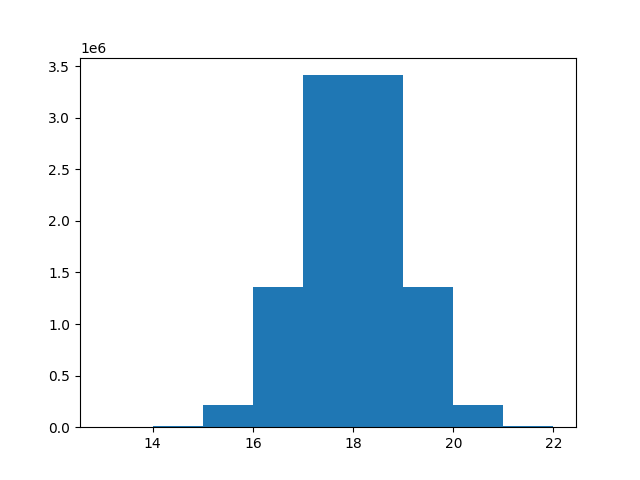
\includegraphics[width=.48\textwidth]{imgs/temp-distribution.png}
    \caption{Temperature distribution}
    \label{fig:temp-distribution}
\end{figure}


%% Secure vault
\section{Secure Vaults implementation}
About the secure vault in the original paper it doesn't define very clearly how it is implemented. What we know from the paper are:
\begin{itemize}
    \item secure vault is a set of \textit{n keys} of \textit{m bits} each;
    \item saved in secure way;
    \item it is updated at the end of the session.
\end{itemize}
We implement a secure vault as an \textbf{array of integers}. On server side, the secure vault is stored in the database (see Listing \ref{lst:sql-table}), instead, on the client we save it in a file that simulates the memory, in both case the secure-vault is in encrypted form. We decided to encrypt it to ensure the confidentiality of the vault in case of memory dump or some vulnerabilities related to the database, even because the security of the protocol is based on keeping the vault secret.

Regarding the update of the secure vault it isn't clearly specified in the original paper, so we implemented as follows:
\begin{enumerate}
    \item compute the HMAC of the actual secure vault value with a given key obtaining a string of \textit{k bits} (depending on the hash algorithm). Our key is the concatenation of the whole data sent during the session;
    \item convert the key in binary;
    \item applied a padding at the end to every key, adding an arbitrary number of zeros, if it is necessary, in order to get partition with dimension \textit{k bits} (even if the dimension of the key is greater than \textit{k bits}, the algorithm splits it in \textit{i} partition of \textit{k bits});
    \item XORed each partition of the secure vault with the HMAC result;
    \item  take the first \textit{m bits} of the XOR results
\end{enumerate}
The point \textit{2} of the update algorithm was necessary because we ensure that the vault to keep a dimension greater than one, otherwise, according to the paper, it is possible to predict the next password/vault configuration easily. 
In Listing \ref{lst:sv-update} is shown the actual implementation

The actual advantage of the update done in the aforementioned way is the fact that the two parts are always synchronize without sending each other any information about the secure-vault.

% valutare se togliere
\begin{lstlisting}[language=Python, basicstyle=\tiny, label= {lst:sv-update}, caption=Secure-vault update]
def update(self, key: bytes) -> list:
    h  = int(hmac.new(key, 
        ",".join(map(str, self._sv)).encode(),
        hashlib.sha512).digest().hex(), 16)
    vault_partitions = self._compute_vault_partition()

    self._sv = [int(bin(h ^ partition)[: self._m + 2], 2) 
                        for partition in vault_partitions]

    return self._sv

def _compute_vault_partition(self) -> list:
    bin_vault = [bin(key).replace("0b", "") for key in self._sv]

    for i, bin_key in enumerate(bin_vault):
        if (reminder := len(bin_key) % PARTITION_DIM) != 0:
            bin_vault[i] = padding(bin_key, len(bin_key) +
                               (PARTITION_DIM - reminder))

    # check if all key has dimension PARTITION_DIM
    for i, key in enumerate(bin_vault):
        if len(key) > PARTITION_DIM:
            bin_vault.pop(i)

            bin_vault = bin_vault + [key[(start := i * 
                        PARTITION_DIM): start + PARTITION_DIM]
                        for i in range(len(key) // PARTITION_DIM)]

    return [int(f"0b{bin_key}", 2) for bin_key in bin_vault]
\end{lstlisting}

%% Tamarin
\section{Tamarin-Prover}
This chapter presents the formal verification of the IoT Authentication Protocol using the Tamarin Prover, a powerful tool for modeling and analyzing cryptographic protocols. The goal is to ensure both authentication and session key secrecy in the implemented system.

Tamarin Prover is designed to verify security protocols by modeling their message flows and analyzing properties such as secrecy and authentication. It uses multiset rewriting rules to represent protocol steps, allowing formal proofs of security guarantees. The protocol rules and the security properties are encoded in a formal language, as demonstrated in this chapter.

Writing the entire protocol in Tamarin involves defining every aspect of the communication process in terms of multiset rewriting rules, facts, and lemmas. Each protocol step is modeled as a rule that consumes and produces facts, representing the states of the protocol participants and the messages exchanged. Fresh values, such as nonces and timestamps, are introduced to ensure security properties like freshness and uniqueness. Additionally, the adversary model is explicitly defined, allowing the prover to test the resilience of the protocol against a powerful attacker capable of intercepting, modifying, and replaying messages. By writing the protocol in this way, it becomes possible to formally verify authentication, key secrecy, and other crucial security properties under a rigorous adversarial model.

The authentication system is modeled with four main protocol steps: client initiation, server response, client verification, and session key establishment. The implementation is expressed as multiset rewriting rules, defining how messages are exchanged and what conditions must be satisfied for a secure session.

\subsection{Function Symbols}
The following function symbols are defined to represent the essential elements of the protocol:
\begin{itemize}
    \item Device id and Session id : Unique identifiers for the device and the session;
    \item c1, c2, r1, r2, t1, and t2 : Fresh nonces and timestamps used to ensure freshness and prevent replay attacks.
    \item Session key : The key that will be established between the client and server.
    \item xor op : A binary operation used to derive the session key from two contributions.
    \item m1, m2, m3, m4 : Protocol messages exchanged between the client and server.
\end{itemize}

\subsection{Protocol Steps}
\begin{enumerate}
    \item Client Initiation (M1): 
            \begin{itemize}
                \item The client generates fresh values for device id and session id.
                \item Sends message m1 containing these identifiers.
            \end{itemize}
    \item Server Response (M2):
            \begin{itemize}
                \item Upon receiving m1, the server generates fresh nonces c1 and r1.
                \item Responds with message m2.
            \end{itemize}
   \item Client Verification and Response (M3):
            \begin{itemize}
                \item The client receives m2, generates new fresh values c2, t1, and r2.
                \item Sends back m3 with these values.
            \end{itemize}
    \item Server Verification and Final Response (M4):
            \begin{itemize}
                \item The server verifies the values and generates a fresh timestamp t2.
                \item Sends message m4 to complete the protocol.
            \end{itemize}
\end{enumerate}

\subsection{Security Check}
To verify the security guarantees of the protocol, two lemmas were defined:
\begin{itemize}
    \item Authentication Agreement: Ensures that if the server finalizes a response, then the client must have initiated the protocol and responded correctly.
    \item Session Key Secrecy: Asserts that once the session key is established, it remains secret and cannot be revealed to an adversary.
\end{itemize}
The formal definitions of these properties in Tamarin guarantee that the protocol achieves mutual authentication and a secure key exchange, critical for IoT environments.

The Tamarin model was executed to verify the specified lemmas. The verification confirmed that:
\begin{itemize}
    \item The protocol successfully enforces authentication, ensuring both the client and server agree on the session parameters.
    \item The established session key remains secret under the defined adversarial model.
\end{itemize}
These results confirm that the IoT authentication system meets its security objectives, offering resilience against replay, impersonation, and key compromise attacks.

%% Conclusions
\section{Conclusions}
In summary, our analysis reveals that the drone’s communication and software design exhibit significant security vulnerabilities. The communication between the remote controller and the drone is entirely unencrypted, leaving the protocol susceptible to eavesdropping and potential manipulation. Furthermore, the companion app available on the Play Store lacks any meaningful security measures.

The app exposes a plethora of sensitive implementation details, including the explicit names of variables used in the code. Additionally, it contains numerous debug logs (Log.d() statements), which greatly simplify the reverse engineering process. These logs provide direct insights into the app's operations and further underscore the lack of attention to security during development.

%% Moreover, our research indicates that the drone does not effectively utilize the control bits available in its communication packets. Altering the value of the XOR byte within the packet does not impact the drone's behavior, suggesting that the drone only evaluates the initial bytes of a packet to determine the command. This design flaw further diminishes the integrity of the protocol and leaves it vulnerable to unauthorized access or spoofing.

These findings collectively highlight the drone's fragile security posture, making it an easy target for exploitation. This serves as a cautionary example of the critical importance of incorporating robust security practices in the development of IoT devices, especially those with wireless communication capabilities.


%% Example
\clearpage

%%%%%%%%%%%%%%%%%%%%%%%%%%%%%%%%%%%%%%%%%
%             BIBLIOGRAPHY
%%%%%%%%%%%%%%%%%%%%%%%%%%%%%%%%%%%%%%%%%

\end{document}